% !TEX root = ../thesis_main.tex



%%%% --- * --- %%%%	
\clearpage
\chapter{Analysis}
\label{analysis_chapter}

Right, so.  Here's how I processed the data into an answer.  In bullet point form, so I don't forget stuff while I'm obsessively trying to phrase everything well.  
\newline

With the Data:
\begin{itemize}
	\item Higher-level data cleaning.  Discard events during parts of the duty cycle when atoms weren't polarized.  Discard events near a recorded spark time.  Discard events when the photoionization laser fires.  Discard events when the LED pulser used to calibrate the scintillators fires.  
	\item Split up runs into sets, to account for changing experimental conditions.  Possibly I should list what the differences between runs were somewhere.  But not in this section.
	\item Using the ``other'' data set with the rMCP:  Measure the trap position/size/velocity/expansion with the rMCP and with the camera.  Necessitates calibrating the rMCP, which is its own whole thing.  Also measure polarization.
		\begin{itemize}
		\item rMCP calibration probably goes in another section.  wev.
		\item We took the mask off before the 2014 run, to give us more detector area.  Use previous reference calibration \emph{with the mask} during the test run in Nov 2013.  The delay line's non-linearities should be the same, assuming we can get the centering the same.  Cables have changed and stuff, so we have to re-center the pre-calibration image to where the old pre-calibration image was.  ...  So, center the new runs w.r.t the old run.
		\item We'll want to make some sum cuts for these things.  We might like them to be identical, or at least identical-ish, but the peaks don't really look the same.  So we'll settle for ``decent sum cuts for all!".  ...  So, apply sum cuts to the new runs and old run.
		\item Calibrate the old run, with the mask.  In fact, I don't remember which order I did things in.  But I have a record of it here, somewhere...
		%	\begin{enumerate}
		%		\item 
		%	\end{enumerate}
		\end{itemize}
	\item Make some more careful cuts to clean the data.  
		\begin{itemize}
		\item Discard events without a ``good'' DSSD hit.  Eliminates vast majority of background 511s.  Necessitates having a definition of what a ``good'' DSSD hit is.  It's subtle enough that we'll want to leave some part of this definition of ``good'' to be varied as a systematic effect.  Notably, we consider energy agreement for each hit pixel, individual strip SNR, and overall DSSD energy threshold.  Also, hit radius w.r.t. center of detector.  This is a lot of stuff, all implemented by Ben -- and it needs to be done fairly early on in data processing in order to keep processing times for everything else manageable.  
		\item Discard events where SOE-Beta TOF falls outside a certain range.  Necessitates picking a ``good'' range.  The precise definition of ``good'' is varied as a systematic.
		\end{itemize}
\end{itemize}

\vspace{24pt}
\vspace{12pt}
With the Simulations:
\begin{itemize}
	\item Update G4 event generator to be able to model non-zero scalar and tensor coupling.  These things show up in $\Abeta$ too, not just in $\bFierz$.  Though, the effects on $\Abeta$ are much smaller.
	\item Run 3 sets of G4 simulations with a bunch of statistics (N events, for data with like N/10 events).  Each one has the same nominal value of $\Abeta$, but with 3 different values of the scalar coupling $C_S$:  zero, and +/-(whatever).  Keep $C_T=0$.  Because reasons, we're not really able to distinguish between $C_S$ and $C_T$ in this experiment anyway, so might as well keep the analysis simple.
	\item Just run one set of 0.02*N events for the two percent branch.  We can't neglect it, but it isn't going to change (much?) when we adjust BSM couplings.
	\item Match cuts in simulated data up to the cuts on experimental data.  Obviously.  DSSD cut, DSSD energy, one hit DSSD, one hit scint.  TOF cut, which requires a whole extra model of background in the TOF spectrum..
		\begin{itemize}
		\item Suppose background in the TOF spectrum is coming from decays of atoms that have gotten themselves stuck to surfaces within the chamber...
		\item Run G4 to get a beta TOF spectrum (w.r.t. the decay)
		\item Run COMSOL (credit to Alexandre) to track low-energy SOEs through the electric field from wherever they started, into the detectors.  Energy spectra from Levinger.
		\item Combine G4 and COMSOL spectra, event-by-event, while requiring that both the beta detector and the eMCP are hit according to the set of random numbers generated by each monte carlo separately.  Then, the beta and SOE will each have a TOF from decay to detector, and subtracting one from the other gives a timing spectrum that can be observed experimentally.  See Fig.~\ref{fig:soetof}.
		\item Upper limit for the fraction of events generated this way can be estimated by assuming that all losses from the trap not due to radioactive decay emerge isotropically from the trap and then stick to whatever chamber wall is in its path.  This upper limit is too big by a factor of 2.
		\end{itemize}
	\item For each of those 3 simulations, sort the ``good'' data according to emission angle relative to the detector.  Do each detector individually.  For both polarizations.
\end{itemize}

\begin{figure}[t!h]
	\centering
	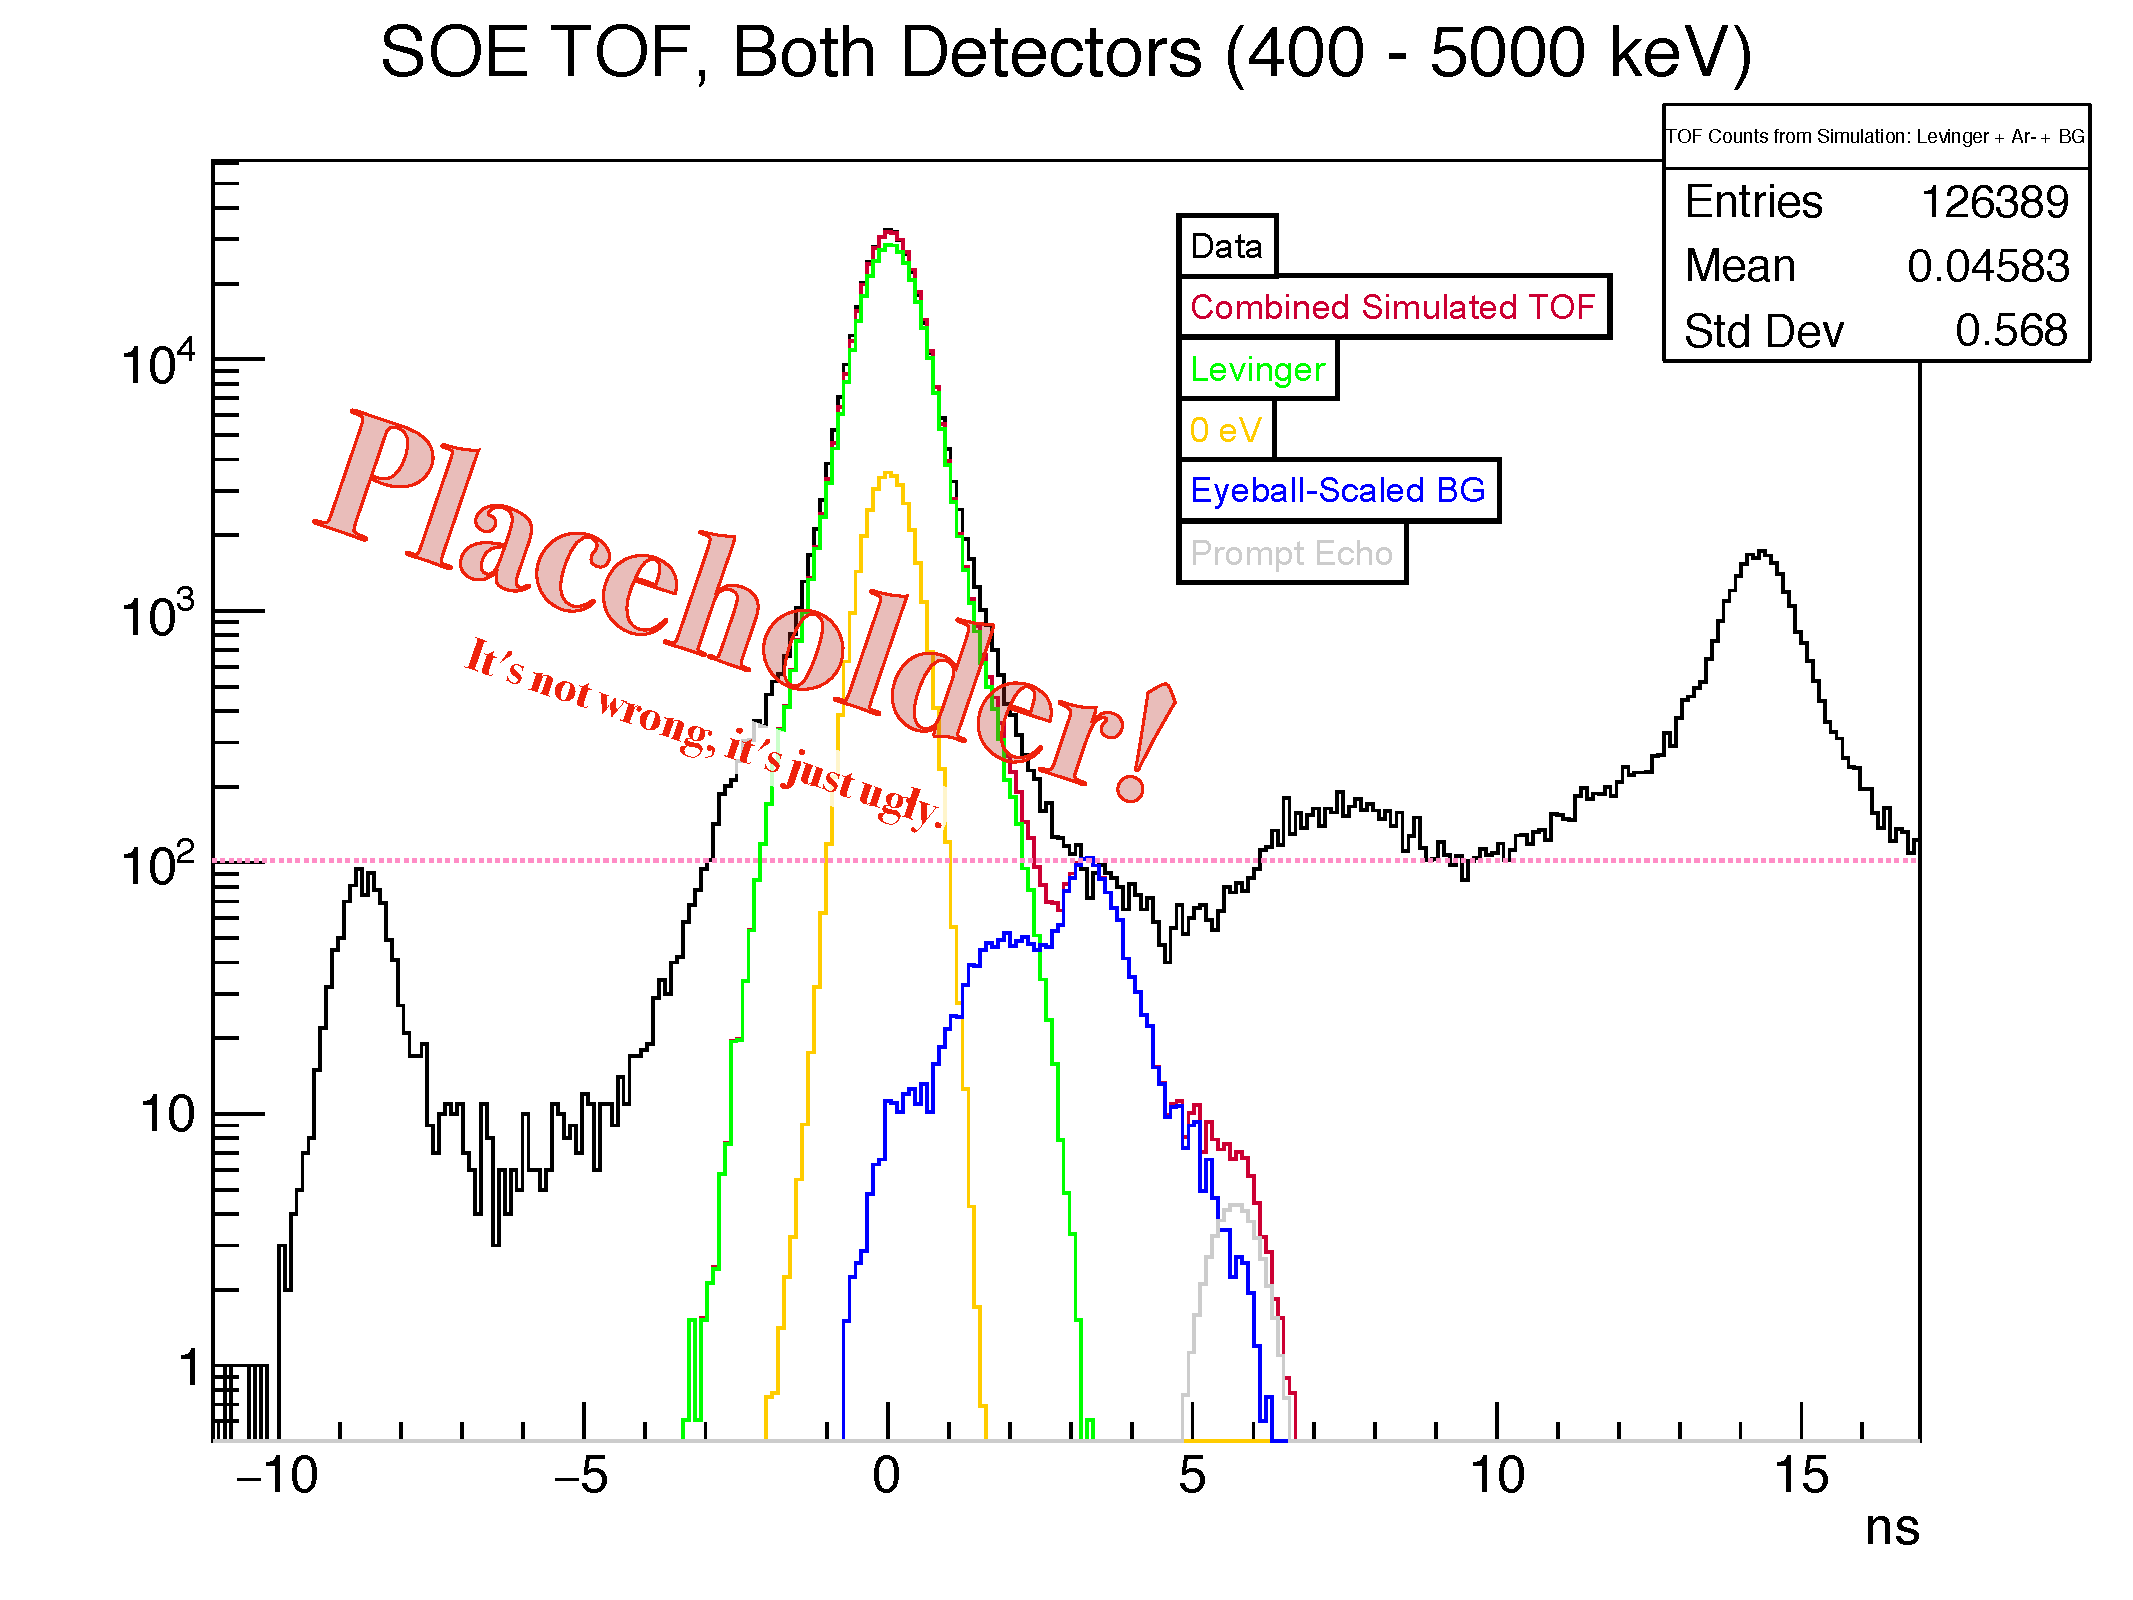
\includegraphics[width=.999\linewidth]
	{Figures/SOETOF_withmodel.pdf}
	\caption{SOE TOF, model and data.  In the end, I cut the data to use only events with a TOF between \comment{A and B.\;\;}  Max. possible background is like a factor of two too big.}	
	\label{fig:soetof}
\end{figure}



